% Print-friendly notes; build presentation.pdf first.
\documentclass[11pt,a4paper]{article}
\usepackage[T1]{fontenc}
\usepackage[utf8]{inputenc}
\usepackage{lmodern}
\usepackage[margin=22mm]{geometry}
\usepackage{graphicx}
\usepackage[hidelinks]{hyperref}
\hypersetup{pdftitle={Presenter notes: the U3 inverse theorem},pdfauthor={Ferran Espuna Bertomeu}}
\usepackage{amsmath,amssymb,mathtools}
\usepackage{tikz}
\usetikzlibrary{arrows.meta,positioning,calc,fit,backgrounds,decorations.pathreplacing}
\definecolor{ink}{HTML}{16324F}
\definecolor{teal}{HTML}{087F8C}
\definecolor{coral}{HTML}{CC5A46}
\definecolor{gold}{HTML}{B47B16}
\definecolor{mist}{HTML}{EAF3F5}
\definecolor{muted}{HTML}{536878}
\newcommand{\E}{\mathbb E}
\newcommand{\T}{\mathbb R/\mathbb Z}
\newcommand{\Z}{\mathbb Z}
\newcommand{\R}{\mathbb R}
\newcommand{\C}{\mathbb C}
\newcommand{\F}{\mathbb F}
\newcommand{\Gh}{\widehat G}
\newcommand{\Bohr}{\operatorname{Bohr}}
\newcommand{\supp}{\operatorname{supp}}
\newcommand{\bb}{\mathcal B}
\newcommand{\abs}[1]{\left|#1\right|}
\newcommand{\norm}[1]{\left\|#1\right\|}
\newcommand{\poly}{\eta^{O(1)}}
\newcommand{\ipoly}{\eta^{-O(1)}}
\newcommand{\JT}[1]{\href{https://arxiv.org/abs/2112.13759}{JT, #1}}
\newcommand{\GT}[1]{\href{https://arxiv.org/abs/math/0503014}{GT, #1}}
\newcommand{\Green}[1]{\href{https://arxiv.org/abs/math/0604089}{Green, #1}}
\tikzset{>=Latex,box/.style={draw=teal,rounded corners=3pt,fill=mist,align=center,inner sep=9pt},arr/.style={->,very thick,teal},smalllabel/.style={font=\scriptsize,text=muted},dot/.style={circle,fill=teal,inner sep=2.2pt}}

\usepackage{enumitem}
\usepackage{array}
\setlist{nosep}
\setlength{\parindent}{0pt}
\setlength{\parskip}{6pt}
\newcounter{talkslide}
\newcommand{\Slide}[4]{%
  \clearpage\stepcounter{talkslide}
  \section*{\arabic{talkslide}. #1}
  \textcolor{teal}{\textbf{Target time: #2}}\par
  \begin{center}\fbox{\includegraphics[page=\arabic{talkslide},width=.79\linewidth]{out/presentation.pdf}}\end{center}
  #4}
\newcommand{\Backup}[4]{\Slide{Backup: #1}{optional}{#3}{#4}}
\begin{document}
\begin{center}
{\LARGE\bfseries Presenter notes}\par\vspace{5mm}
{\Large The $U^3$ inverse theorem on arbitrary finite abelian groups}\par\vspace{3mm}
Ferran Espu\~na Bertomeu\quad Kopp, October 4--9, 2026
\end{center}
The audience deck follows the assigned Fourier-analytic proof of \JT{Theorem 1.6}.
The numbered notes below are the spoken route; the preparation appendix supplies
derivations and source checks for rehearsal and questions. It is not additional
material to deliver in the 45-minute slot.

\textbf{Pacing.} The 27 substantive slides total 40 minutes 45 seconds, leaving
4 minutes 15 seconds for pauses and questions. The references slide and five
backup slides have no scheduled speaking time.

\begin{center}
\begin{tabular}{lll}
Slides & Topic & Cumulative target\\\hline
1--5 & Statement and proof route & 5:30\\
6--12 & Lemma 2.5: organising frequencies & 17:00\\
13--17 & Lemma 2.6: symmetry & 25:00\\
18--24 & Example 2.3; lifting and integration & 34:30\\
25--27 & Finish Theorem 1.6 & 40:45
\end{tabular}
\end{center}

\textbf{If running late.} On slide 10 give the collision-removal idea and omit
the cardinality calculation (save 45 seconds). On slide 15 state local
Bogolyubov and give the three-arrow argument (save 45 seconds). On slide 24
use only the parabola, leaving the $\Z/2\Z$ check for questions (save 30 seconds).
Keep the theorem statements, the graph-to-$M$ argument, the real midpoint,
and the final Fourier step.

\textbf{Conventions.} $e(t)=\exp(2\pi it)$, all averages are normalised,
$\widehat f(\xi)=\E_x f(x)e(-\xi\cdot x)$, and $b$ denotes changing
1-bounded functions of exactly the displayed arguments. Polynomial losses
are always in $\eta$, independent of $G$. A locally linear map means vanishing
second differences on every parallelogram in its domain; the constructed $M$
also satisfies $M(0)=0$.

% Each slide and its spoken notes have one shared source.
\Slide{The $U^3$ inverse theorem}{0:30}{
\vspace{3mm}
{\LARGE\bfseries Arbitrary finite abelian groups}\par\vspace{4mm}
{\large From Fourier coefficients to local quadratics}\par\vspace{8mm}
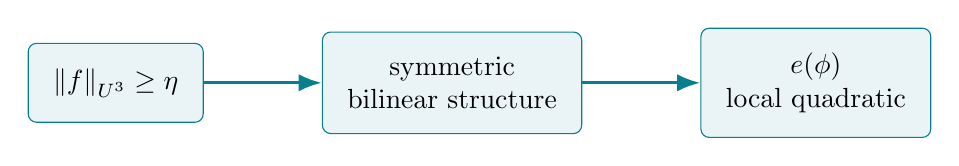
\begin{tikzpicture}
\node[box] (a) {$\norm{f}_{U^3}\geq\eta$};
\node[box,right=15mm of a] (b) {symmetric\\bilinear structure};
\node[box,right=15mm of b] (c) {$e(\phi)$\\local quadratic};
\draw[arr] (a)--(b);\draw[arr] (b)--(c);
\end{tikzpicture}
\vfill
Ferran Espu\~na Bertomeu\quad {\small UAM}\par
{\small Kopp Summer School\enspace $\cdot$\enspace October 4--9, 2026}
\source{After Asgar Jamneshan and Terence Tao (2023), Theorem 1.6.}
}{
The aim is to prove a quantitative inverse theorem uniformly over all finite
abelian groups. A large $U^3$ norm produces locally quadratic structure.
We will organise derivative frequencies, symmetrise them, then integrate.
The new algebraic issue is that division by two and global extension can fail.
Two explicitly stated algebraic lemmas handle this. The talk uses the additive
combinatorial input from Talks 3--5, but explains exactly how it is applied.
}

\Slide{A quadratic phase has linear derivatives}{1:00}{
\begin{columns}[c]
\column{.40\textwidth}
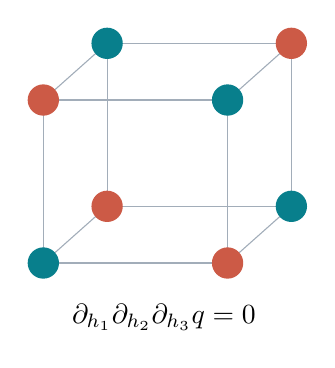
\begin{tikzpicture}[scale=.9]
\foreach \x/\y/\n in {0/0/000,2.6/0/100,0/2.3/010,2.6/2.3/110,.9/.8/001,3.5/.8/101,.9/3.1/011,3.5/3.1/111}{\coordinate (\n) at (\x,\y);}
\foreach \a/\b in {000/100,000/010,100/110,010/110,001/101,001/011,101/111,011/111,000/001,100/101,010/011,110/111}{\draw[ink!40] (\a)--(\b);}
\foreach \n in {000,110,101,011}{\node[circle,fill=teal,inner sep=4pt] at (\n) {};}
\foreach \n in {100,010,001,111}{\node[circle,fill=coral,inner sep=4pt] at (\n) {};}
\node[below=4mm] at (1.7,0) {$\partial_{h_1}\partial_{h_2}\partial_{h_3}q=0$};
\end{tikzpicture}
\column{.59\textwidth}
\[\Delta_h f(x):=f(x+h)\overline{f(x)}\]
\[f=e(q)\quad\Longrightarrow\quad\Delta_h f(x)=e(q(x+h)-q(x))\]
\[\boxed{\norm{f}_{U^3}^8=\E_h\norm{\Delta_h f}_{U^2}^4}\]
\tagline{Large $U^3$ $\Rightarrow$ many linear derivatives.}
\end{columns}
}{
Recall the derivative identity from the earlier talks. In the cube picture,
teal and coral vertices have opposite signs in the alternating sum. A
quadratic polynomial has zero third difference, so its phase has $U^3$ norm
one. For a general 1-bounded function, the displayed identity reduces the
problem to the $U^2$ inverse theorem for many derivatives. The difficulty is
making their frequencies depend linearly on the increment. We use the
forward multiplicative derivative here; additive derivatives can equivalently
be defined by $\partial_h q(x)=q(x+h)-q(x)$.
}

\Slide{The neighbourhood where algebra works}{1:30}{
\begin{columns}[c]
\column{.36\textwidth}
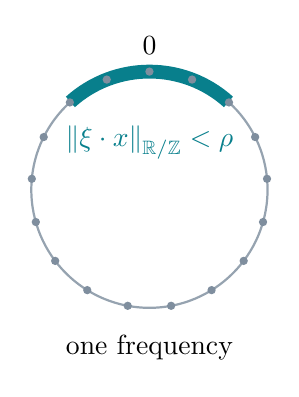
\begin{tikzpicture}[scale=.75]
\draw[ink!45,thick] (0,0) circle (2);
\draw[teal,line width=5pt] (48:2) arc (48:132:2);
\foreach \k in {0,...,16}{\fill[ink!55] ({90-360*\k/17}:2) circle (2pt);}
\node[above] at (90:2.12) {$0$};
\node[teal] at (0,.8) {$\norm{\xi\cdot x}_{\T}<\rho$};
\node[below] at (0,-2.3) {one frequency};
\end{tikzpicture}
\column{.63\textwidth}
\[\norm{x}_S:=\max_{\xi\in S}\norm{\xi\cdot x}_{\T},\qquad
\bb_\rho:=\Bohr(S,\rho).\]
\begin{block}{Local polynomial}
A map $q:U\to\T$ is locally quadratic if every third additive
difference vanishes whenever all eight vertices lie in $U$.
\end{block}
\small
Locally linear: every second difference vanishes.\par\medskip
Regularity: $|\bb_{(1+\kappa)\rho}|=(1+O(|S||\kappa|))|\bb_\rho|$.
\tagline{Small shifts change averages only slightly.}
\end{columns}
\source{Definitions: \JT{1.4--1.5}. Regular radii and shift estimates: \GT{Lemmas 8.2 and 4.2}.}
}{
A Bohr set is the simultaneous inverse image of small arcs around zero under
a finite list of characters. The picture shows one arc. It need not be a
subgroup, so every local identity comes with domain conditions. In particular,
locally quadratic means vanishing on every cube whose vertices remain in the
domain, not just cubes based at zero. For a locally bilinear form, additivity
in either variable is required whenever the summands and their sum remain
in the domain.

Regularity says that a thin change in radius changes the size by only
$O(|S||\kappa|)$. Hence translation by $t$ with $\norm{t}_S\leq\varepsilon\rho$
changes a bounded average over $\bb_\rho$ by $O(|S|\varepsilon)$.
We use the standard existence of a regular radius in $[r,2r]$.
The precise statements and the elementary boundary argument are in backup
slide 1 and the preparation appendix. Explain the purpose here, not the
regular-radius proof.
}

\Slide{The target: one local quadratic, many translates}{2:00}{
\begin{block}{Theorem 1.6 (Jamneshan--Tao)}
Let $G$ be a finite abelian group, $0<\eta\leq\tfrac12$, and
$f:G\to\C$ satisfy $|f|\leq1$ and $\norm{f}_{U^3(G)}\geq\eta$.
There exist a regular Bohr set $\bb_\rho=\Bohr(S,\rho)$ with
\[|S|\ll\ipoly,\qquad \exp(-\ipoly)\ll\rho\leq\tfrac1{100},\]
a locally quadratic map $\phi:\bb_\rho\to\T$, and a map
$\xi:G\to\Gh$ such that
\[\boxed{\E_{x\in G}\abs{\E_{h\in\bb_\rho}
f(x+h)e(-\phi(h)-\xi(x)\cdot h)}\gg\poly.}\]
\end{block}
\tagline{Uniform in $G$\qquad including even and mixed torsion.}
\source{\JT{Theorem 1.6}.}
}{
Read the hypotheses and explain the conclusion without reading every symbol
twice. There is a single Bohr neighbourhood and a single local quadratic
$\phi$. The linear correction $\xi(x)$ may depend arbitrarily on the base
point. The absolute value is inside the average over base points; the theorem
therefore gives useful correlation on a positive proportion of translates.

The dimension is polynomial in $1/\eta$, the radius may be exponentially
small, and the correlation is still polynomial in $\eta$. This distinction
will matter when we shrink the domain: we cannot just discard all but an
exponentially small subset of an average. All constants are independent of
the order and torsion of $G$. Throughout the proof, $b$ denotes a changing
1-bounded function of exactly its displayed variables, and all averages
are normalised.
}

\Slide{The proof in four moves}{0:30}{
\centering\vspace{3mm}
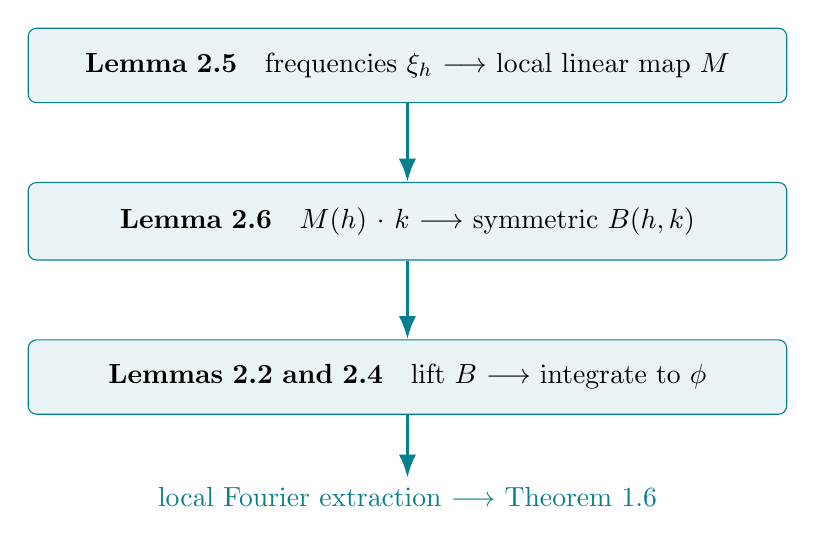
\begin{tikzpicture}[node distance=10mm]
\node[box,text width=9cm] (a) {\textbf{Lemma 2.5}\quad frequencies $\xi_h$ $\longrightarrow$ local linear map $M$};
\node[box,text width=9cm,below=of a] (b) {\textbf{Lemma 2.6}\quad $M(h)\cdot k$ $\longrightarrow$ symmetric $B(h,k)$};
\node[box,text width=9cm,below=of b] (c) {\textbf{Lemmas 2.2 and 2.4}\quad lift $B$ $\longrightarrow$ integrate to $\phi$};
\node[below=8mm of c,text=teal] (d) {local Fourier extraction $\longrightarrow$ Theorem 1.6};
\draw[arr] (a)--(b);\draw[arr] (b)--(c);\draw[arr] (c)--(d);
\end{tikzpicture}
}{
This is the whole route. We prove the analytic steps, state the precise
combinatorial inputs, and illustrate the two algebraic black boxes using
Example 2.3. The graph construction is the longest part to explain because
it is where independent Fourier coefficients become an algebraic object.
}

\Slide{Lemma 2.5: a coherent frequency map}{1:00}{
\begin{block}{Lemma 2.5 (Jamneshan--Tao)}
Under the hypotheses of Theorem 1.6, there exist a regular Bohr set
$\bb_\rho=\Bohr(S,\rho)$ with $|S|\ll\ipoly$ and
$c\leq\rho\leq\tfrac18$ for an absolute $c>0$, a locally linear map
$M:\bb_{2\rho}\to\Gh$, and 1-bounded functions $b_1,b_2$ such that
\[\abs{\E_{\substack{x\in G\\h\in\bb_\rho}}
b_1(h)b_2(x)f(x+h)e(-M(h)\cdot x)}\gg\poly.\]
\end{block}
\vspace{3mm}
\centering
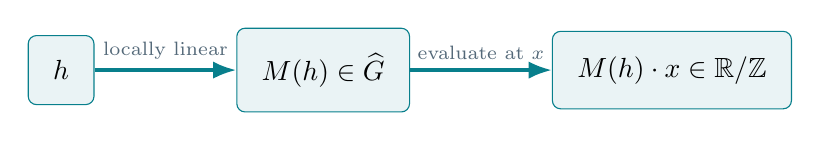
\begin{tikzpicture}
\node[box] (a) {$h$};\node[box,right=18mm of a] (b) {$M(h)\in\Gh$};\node[box,right=18mm of b] (c) {$M(h)\cdot x\in\T$};
\draw[arr] (a)--node[above,smalllabel]{locally linear}(b);
\draw[arr] (b)--node[above,smalllabel]{evaluate at $x$}(c);
\end{tikzpicture}
\source{\JT{Lemma 2.5}; adapts \GT{Propositions 5.1, 5.4, 9.1 and 9.3}.}
}{
State the lemma fully. The desired phase is linear in $x$ and locally linear
in $h$. The two separate bounded factors are allowed, but a factor depending
jointly on $x$ and $h$ would make the conclusion meaningless. We will keep
track of those dependencies. Our construction has $M(0)=0$.
The radius can be chosen between $1/16$ and $1/8$ in the construction below.
The notation $1\ll\rho$ in the paper means a positive absolute lower bound,
not a radius greater than one. The adaptation from Green--Tao is to construct
$M$ directly instead of writing a frequency as $2M$: division by two in
$\Gh$ is not available for arbitrary groups.
}

\Slide{Differentiate, then use ordinary Fourier analysis}{1:30}{
\[\eta^8\leq\E_h\norm{\Delta_hf}_{U^2}^4
=\E_h\sum_{\xi\in\Gh}|\widehat{\Delta_h f}(\xi)|^4\]
\[\sum_\xi|\widehat{\Delta_h f}(\xi)|^2\leq1
\quad\Longrightarrow\quad
\norm{\Delta_hf}_{U^2}^4\leq\max_\xi|\widehat{\Delta_hf}(\xi)|^2.\]
\begin{block}{Many good increments}
There are $H\subseteq G$ with $|H|\geq\eta^8|G|/2$ and frequencies
$\xi_h\in\Gh$ such that, for every $h\in H$,
\[\abs{\E_x f(x+h)\overline{f(x)}e(-\xi_h\cdot x)}\geq\eta^4/\sqrt2.\]
\end{block}
\tagline{Next: force additive relations among the $\xi_h$.}
\source{\GT{Proposition 5.1, first step}.}
}{
The $U^2$ identity is Parseval followed by the Fourier formula for $U^2$.
For each $h$, the fourth-power sum is at most the largest squared coefficient
times the squared-coefficient sum, which is at most one. Define $H$ by
requiring that maximum squared coefficient to be at least $\eta^8/2$.
The contribution outside $H$ is at most $\eta^8/2$, hence $|H|/|G|\geq\eta^8/2$.
Choose a maximizing frequency for each good increment. Its coefficient is
at least $\eta^4/\sqrt2$.

This only creates a collection of frequencies. There is no reason yet that
$\xi_{h+k}=\xi_h+\xi_k$. We next use that all these coefficients arise from
derivatives of the same function. No combinatorial theorem has been used yet.
}

\Slide{Cauchy--Schwarz detects parallelograms}{2:00}{
\begin{columns}[c]
\column{.43\textwidth}
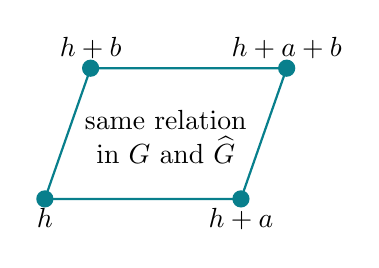
\begin{tikzpicture}[scale=.83]
\coordinate (a) at (0,0);\coordinate (b) at (3,0);
\coordinate (c) at (.7,2);\coordinate (d) at (3.7,2);
\draw[teal,thick] (a)--(b)--(d)--(c)--cycle;
\foreach \v in {a,b,c,d}{\node[dot] at (\v) {};}
\node[below] at (a) {$h$};\node[below] at (b) {$h+a$};
\node[above] at (c) {$h+b$};\node[above] at (d) {$h+a+b$};
\node[align=center] at (1.85,.95) {same relation\\in $G$ and $\Gh$};
\end{tikzpicture}
\column{.56\textwidth}
\[\Gamma:=\{(h,\xi_h):h\in H\}\]
\[\xi_h+\xi_{h+a+b}=\xi_{h+a}+\xi_{h+b}\]
\begin{center}\small for $\gg\eta^{64}|G|^3$ parallelograms in $H$\end{center}
\[\boxed{E(\Gamma)\gg\eta^{64}|G|^3}\]
\small $E(\Gamma)=\#\{\gamma_1+\gamma_2=\gamma_3+\gamma_4\}$.
\end{columns}
\tagline{Square correlation $\to$ two Cauchy--Schwarz steps $\to$ orthogonality.}
\source{\GT{Proposition 5.1, equations (5.4)--(5.8)}.}
}{
Write $a_h(x)=\Delta_h f(x)$. Squaring its Fourier coefficient introduces
a displacement $k$:
$|\widehat a_h(\xi_h)|^2=\E_{x,k}a_h(x)\overline{a_h(x+k)}e(\xi_h\cdot k)$.
The product of the four $f$ factors separates as $u(x+h,k)v(x,k)$,
with both functions 1-bounded. Averaging over good $h$ gives a trilinear
average of size at least $\eta^{16}/4$.

Apply Cauchy--Schwarz to eliminate $v(x,k)$, introducing a second increment
$h+a$. Change variables to $y=x+h$; the remaining bounded factors no
longer depend on $h$. A second Cauchy--Schwarz removes them and introduces
$h+b$. What remains is the phase with frequency
$\xi_h-\xi_{h+a}-\xi_{h+b}+\xi_{h+a+b}$, with the four indicators of $H$.
Averaging in $k$ gives exactly the indicator that this frequency is zero.
The lower bound has been squared twice, giving $\eta^{64}/256$.
This proves the energy claim, not just an analogy with a quadratic.
The preparation appendix gives the complete two-line Cauchy--Schwarz calculation.
}

\Slide{The combinatorial input: what each theorem supplies}{1:30}{
\begin{block}{Balog--Szemer\'edi--Gowers [black box]}
If a finite nonempty set $A$ in an abelian group satisfies
$E(A)\geq |A|^3/K$, $K\geq1$, then some $A'\subseteq A$ satisfies
$|A'|\geq cK^{-C}|A|$ and $|A'-A'|\leq CK^C|A'|$,
for absolute constants $c,C>0$.
\end{block}
\begin{block}{Pl\"unnecke [black box]}
If $|A-A|\leq L|A|$ for a finite nonempty set $A$ in an abelian group,
then $|kA-\ell A|\leq L^{k+\ell}|A|$ for all integers $k,\ell\geq1$.
\end{block}
\[E(\Gamma)\text{ large}\quad\Longrightarrow\quad
\boxed{|\Gamma'|\geq |G|/K,\quad |9\Gamma'-8\Gamma'|\leq K|G|,\quad K\ll\ipoly.}\]
\source{\GT{Theorems 5.2--5.3 and Proposition 5.4}. These are inputs from Talks 3--5.}
}{
State the two inputs, including their polynomial quantitative bounds.
BSG upgrades many additive quadruples to a large subset of small doubling.
Pl\"unnecke then controls the particular long sumset $9\Gamma'-8\Gamma'$.
We enlarge one polynomial parameter $K$ to cover both inequalities in the box.
Since every subset of a graph is still a graph, all original derivative
correlations are retained.

The important distinction is that small doubling does not imply that
$2\Gamma'-2\Gamma'$ is a graph. It may have several points above one
increment. Nor is $\Gamma$ dense in $G\times\Gh$: its size is on the scale
of $|G|$, not $|G|^2$. Bogolyubov will later be used on a subset of $G$.
The numbers nine and eight are bookkeeping for the collision argument on
the next slide, not mysterious structural constants.
}

\Slide{Remove the vertical collisions}{2:00}{
\begin{columns}[c]
\column{.42\textwidth}
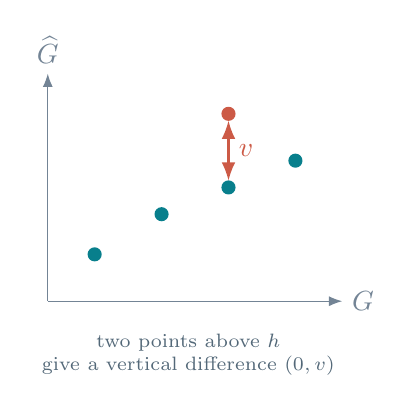
\begin{tikzpicture}[scale=.85]
\draw[->,ink!60] (0,0)--(4.4,0) node[right] {$G$};
\draw[->,ink!60] (0,0)--(0,3.4) node[above] {$\Gh$};
\foreach \x/\y in {.7/.7,1.7/1.3,2.7/1.7,3.7/2.1}{\fill[teal] (\x,\y) circle(3pt);}
\fill[coral] (2.7,2.8) circle(3pt);
\draw[<->,coral,thick] (2.7,1.8)--node[right] {$v$}(2.7,2.7);
\node[align=center,smalllabel] at (2.1,-.8) {two points above $h$\\give a vertical difference $(0,v)$};
\end{tikzpicture}
\column{.57\textwidth}
\[V:=\{v:(0,v)\in8\Gamma'-8\Gamma'\},\qquad |V|\leq K^2.\]
\small Choose $O(\log K)$ characters separating $V\setminus\{0\}$.
Keep frequencies in one small torus cube.
\[\Gamma''\subseteq\Gamma',\qquad |\Gamma''|\geq K^{-O(1)}|G|\]
\[\boxed{(8\Gamma''-8\Gamma'')\cap(\{0\}\times\Gh)=\{(0,0)\}.}\]
\tagline{$4\Gamma''-4\Gamma''$ is a graph.}
\end{columns}
\source{\GT{Lemma 9.2; separation lemma 8.3}. Proof unpacked in the notes.}
}{
Let $V$ be the possible vertical differences. Since $\Gamma'$ is a graph,
all $|\Gamma'||V|$ sums in $\Gamma'+(\{0\}\times V)$ are distinct. This set
lies inside $9\Gamma'-8\Gamma'$, so $|V|\leq K^2$.

Use $O(\log(2|V|))$ characters on $\Gh$ to ensure that the only
$v\in V$ with all character values within $1/4$ of zero is $v=0$.
Why possible? A random character excludes at least a third of the remaining
nonzero points on average; iterate. Partition the resulting torus into
half-open cubes of side $1/128$. One cube captures a polynomial proportion
of $\Gamma'$; call this subset $\Gamma''$.

An eight-minus-eight sum of frequencies in that cube has each tested
coordinate of size less than $16/128<1/4$. If its first coordinate is zero,
its frequency also belongs to $V$, hence is zero. Two points of
$4\Gamma''-4\Gamma''$ with the same first coordinate have just such a
vertical difference. They must therefore coincide. This is the graph
property we needed. The discarded subset costs only a power of $K$.
}

\Slide{A Bohr set inside the graph gives $M$}{2:00}{
\begin{block}{Bogolyubov [black box]}
If $A\subseteq G$ has density $\delta>0$ in a finite abelian group,
there is $S\subseteq\Gh$ with $|S|\leq2\delta^{-2}$ such that
$\Bohr(S,\tfrac14)\subseteq 2A-2A$.
\end{block}
\small Apply to $H''=\pi_G(\Gamma'')$, with $\delta\gg\poly$.
\[\bb_{1/4}\subseteq 2H''-2H'',\qquad
(h,M(h))\in2\Gamma''-2\Gamma''\quad(h\in\bb_{1/4}).\]
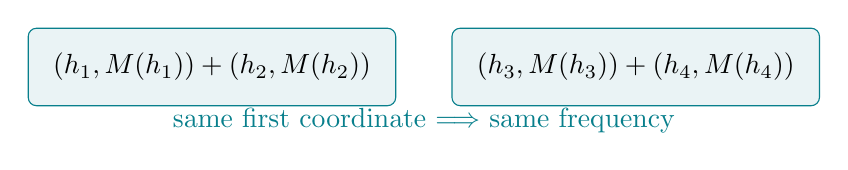
\begin{tikzpicture}
\node[box] (a) {$(h_1,M(h_1))+(h_2,M(h_2))$};
\node[box,right=7mm of a] (b) {$(h_3,M(h_3))+(h_4,M(h_4))$};
\node[below=4mm of $(a)!0.5!(b)$,text=teal] {same first coordinate $\Longrightarrow$ same frequency};
\end{tikzpicture}
\[h_1+h_2=h_3+h_4\quad\Longrightarrow\quad
M(h_1)+M(h_2)=M(h_3)+M(h_4).\]
\source{\GT{Lemma 6.3 and Proposition 9.1}, with the factor $2$ removed as in \JT{Lemma 2.5}.}
}{
Bogolyubov is applied to the projection $H''$, whose density is polynomial
in $\eta$. This produces a Bohr set of polynomial rank and constant radius.
Every point $h$ in it has at least one lift to $2\Gamma''-2\Gamma''$;
the graph property makes that lift unique, defining $M(h)$.

Take any four points of the Bohr set with equal pair sums. Both sums of
their lifts lie in $4\Gamma''-4\Gamma''$. Its graph property forces their
frequency coordinates to agree. This proves vanishing second differences
on every parallelogram in the domain, the full definition of local linearity.
Also $M(0)=0$, because the zero pair lies in the difference set. In
particular $M(h+k)=M(h)+M(k)$ whenever all three points are in the domain.

There is no requirement that the common sum itself lie in the Bohr set in
the four-point argument. This is why four copies, rather than two, were
needed in the graph refinement. We have produced $M$, but must still
recover correlation with $f$.
}

\Slide{Recover the correlation: an affine patch}{1:30}{
\small Choose regular $\rho\in[1/16,1/8]$ and $x_0$ with
$A:=\{h\in\bb_\rho:x_0+h\in H''\}$ of relative density $\gg\poly$.
\[\xi_{x_0+h}-\xi_{x_0+h'}=M(h-h')=M(h)-M(h')\]
\[\boxed{\xi_{x_0+h}=\xi_0+M(h)\qquad(h\in A).}\]
\[\E_{h\in\bb_\rho}\mathbf1_A(h)
\abs{\E_x f(x+x_0+h)\overline{f(x)}e(-[\xi_0+M(h)]\cdot x)}\gg\poly.\]
\tagline{Align phases in $h$\quad$+$\quad shift $x$\quad$=$\quad Lemma 2.5.}
\source{\GT{end of Proposition 9.1 and Proposition 9.3}; \JT{Lemma 2.5}.}
}{
Averaging $\mathbf1_{H''}(x_0+h)$ over $x_0$ gives the global density of
$H''$, so some translate contains a polynomial relative density of good
increments. For $h,h'\in A$, the pair
$(h-h',\xi_{x_0+h}-\xi_{x_0+h'})$ belongs to $\Gamma''-\Gamma''$.
Uniqueness of the lift and local linearity give the first display. Fixing
$h'$ shows that the original frequencies agree with $\xi_0+M(h)$ on $A$.

All these frequencies still have their original large Fourier coefficients.
Choose a unit complex number for each $h\in A$ to align its coefficient,
and zero outside $A$. Finally put $u=x+x_0$. The factor
$\overline{f(u-x_0)}e(-\xi_0\cdot u)$ depends only on $u$; the factor
$e((\xi_0+M(h))\cdot x_0)$ depends only on $h$. Absorb them separately
into $b_2(u)$ and $b_1(h)$. We obtain exactly Lemma 2.5 with the original
$f(u+h)$. This completes the lemma, including its correlation conclusion.
}
% --------------------------------------------------------------------------
% The remaining slides continue below the frequency-map argument.
\Slide{Lemma 2.6: make the bilinear form symmetric}{1:00}{
\begin{block}{Lemma 2.6 (Jamneshan--Tao)}
Under the hypotheses of Theorem 1.6, there exist a regular Bohr set
$\bb_\rho=\Bohr(S,\rho)$ with $|S|\ll\ipoly$ and
$\poly\ll\rho\leq\tfrac18$, a symmetric locally bilinear map
$B:\bb_{2\rho}\times\bb_{2\rho}\to\T$, and 1-bounded functions
$b_1,b_2$ such that
\[\abs{\E_{\substack{x\in G\\h,k\in\bb_\rho}}
b_1(x,h)b_2(x,k)f(x+h+k)e(-B(h,k))}\gg\poly.\]
\end{block}
\[D(y,z):=M(y)\cdot z-M(z)\cdot y\]
\tagline{Control the antisymmetric defect $D$, then take a real midpoint.}
\source{\JT{Lemma 2.6}; symmetry argument adapted from \GT{Lemma 9.4}.}
}{
The form $M(h)\cdot k$ is locally bilinear, but need not be symmetric.
A quadratic second derivative is symmetric, so this is the next obstruction.
Read the new lemma: the two bounded factors may share $x$, but one depends
on $h$ and the other on $k$. That separation is essential.

Define the antisymmetric defect $D$. We first prove it is small on a smaller
Bohr set, using the fact that $M$ came from derivatives of one function.
Then we correct the form to exact symmetry by lifting the small defect to
the reals. We do not divide a character by two. The next three slides give
the symmetry argument and the fourth transfers the correlation.
}

\Slide{Symmetry starts with one more Cauchy--Schwarz}{2:00}{
\small Localise $x$ to a small regular Bohr set $U$; write $P$ for the larger one.
\[\abs{\E_{h\in P,\,x\in U} b(h)b(x+h)b(x)e(-M(h)\cdot x)}\gg\poly\]
\begin{center}\textcolor{teal}{$\downarrow$\quad Cauchy--Schwarz in $h$; put $w=x+y+h$}\end{center}
\[\abs{\E_{x,y\in U}u(x)v(y)e(D(x,y))}\gg\poly\]
\begin{center}\textcolor{teal}{$\downarrow$\quad Cauchy--Schwarz; average in $y_0$}\end{center}
\[\boxed{\abs{\E_{x\in U}e(D(x,y_0-y))}\geq\tau
\quad(y\in A),\qquad |A|\geq\tau|U|,\quad\tau\gg\poly.}\]
\source{\GT{Lemma 9.4, through (9.17)}, omitting the factor $2$ as instructed in \JT{Lemma 2.6}.}
}{
Localisation costs no density: average over translates of a small regular
Bohr set $U$, then fix one translate on which the original correlation
survives. Its centre is absorbed into bounded factors.
Square the correlation and apply Cauchy--Schwarz in $h$ to remove $b(h)$.
There are now two variables $x,y\in U$. Set $w=x+y+h$ and expand
$M(w-x-y)$ using local linearity. All terms except
$M(x)\cdot y-M(y)\cdot x$ depend on only $(w,x)$ or $(w,y)$; their signs
can be absorbed into those bounded factors. If the opposite sign occurs,
swap $x,y$.

The $w$ domain is $P+x+y$. Regularity of $P$ allows us to replace this by
$P$, since $U$ is much smaller. Fix a $w$ retaining correlation. This gives
the middle display with two separate bounded functions. Cauchy--Schwarz
removes $u(x)$, leaving the mean over $y,y'$ of the absolute value of
$\E_x e(D(x,y'-y))$. Fix $y'=y_0$, then keep a dense set $A$ where that
absolute value is large. All losses remain polynomial.
}

\Slide{Large local Fourier means force a small defect}{2:00}{
\begin{block}{Local Bogolyubov [black box]}
Let $U=\Bohr(S,r)$ be regular, $d=\max(1,|S|)$, and
$A\subseteq U$ have relative density $\delta>0$. There is
$T\subseteq\Gh$ with $|T|\leq C\delta^{-3}$ such that
\[\Bohr(S\cup T,c\delta^6r/d)\subseteq2A-2A,\]
where $c,C>0$ are absolute constants.
\end{block}
\begin{center}
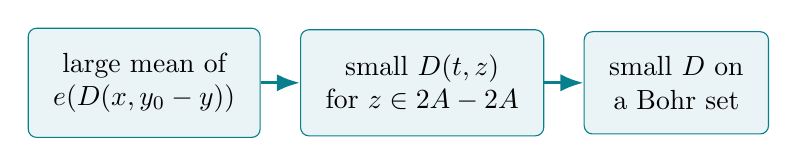
\begin{tikzpicture}[node distance=5mm]
\node[box] (a) {large mean of\\$e(D(x,y_0-y))$};
\node[box,right=of a] (b) {small $D(t,z)$\\for $z\in2A-2A$};
\node[box,right=of b] (c) {small $D$ on\\a Bohr set};
\draw[arr] (a)--(b);\draw[arr] (b)--(c);
\end{tikzpicture}
\end{center}
\[\norm{D(t,z)}_{\T}\ll\ipoly\norm{t}_{S\cup T}.\]
\source{Local Fourier decay: \GT{Lemma 8.4} (proved in notes). Local Bogolyubov: \GT{Lemma 8.8}.}
}{
The elementary analytic fact is this: if a locally additive phase $\ell$ on
$\Bohr(S,2r)$ has mean of magnitude at least $\tau$ on a regular
$U=\Bohr(S,r)$, then
$\norm{\ell(t)}_{\T}\leq C d\norm{t}_S/(r\tau^2)$ for $t\in U$.
Brief proof: average small translations $x+nt$; regularity preserves the
large mean, while local linearity factors off $e(n\ell(t))$. A geometric
sum cannot be large unless $\ell(t)$ is close to an integer.

Apply this to $\ell(x)=D(x,y_0-y)$ for every $y\in A$ from the previous
slide. Taking two differences cancels $y_0$ and gives the same estimate,
with a factor four, for all $z\in2A-2A$. The local Bogolyubov theorem then
places a Bohr set of polynomial rank and polynomial radius inside this
set. Restrict both variables to it. This proves the displayed defect
bound. Shrinking once more makes it smaller than any prescribed power
of $\eta$.

Local, rather than global, Bogolyubov is essential: $A$ is dense relative
to $U$, whose global density may be exponentially small. The preparation
appendix explains its Fourier proof and the local Bessel input.
}

\Slide{A small defect has a real half}{1:30}{
\begin{columns}[c]
\column{.37\textwidth}
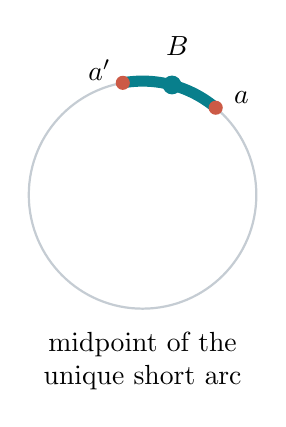
\begin{tikzpicture}[scale=.85]
\draw[ink!25,thick] (0,0) circle (1.7);
\draw[teal,line width=4pt] (50:1.7) arc (50:100:1.7);
\fill[coral] (50:1.7) circle(3pt);\fill[coral] (100:1.7) circle(3pt);
\fill[teal] (75:1.7) circle(4pt);
\node[right] at (50:1.9) {$a$};\node[left] at (100:1.9) {$a'$};
\node[above] at (75:2.0) {$B$};
\node[align=center,below] at (0,-1.9) {midpoint of the\\unique short arc};
\end{tikzpicture}
\column{.62\textwidth}
\small On a sufficiently small doubled Bohr set:
\[D(y,z)=d(y,z)\pmod1,\qquad |d(y,z)|<\varepsilon<\tfrac1{10}.\]
\[\boxed{B(y,z):=M(y)\cdot z-\tfrac12d(y,z).}\]
\[B(y,z)=B(z,y),\qquad B\ \text{locally bilinear}.\]
\[|e(-M(y)\cdot z)-e(-B(y,z))|\leq\pi\varepsilon.\]
\end{columns}
\source{\JT{Lemma 2.6, equation (25)}.}
}{
Let $d(y,z)$ be the unique real representative of $D(y,z)$ in
$(-\varepsilon,\varepsilon)$. Its local additivity is exact: the difference
$d(y_1+y_2,z)-d(y_1,z)-d(y_2,z)$ is an integer with absolute value below
$3\varepsilon<1$, hence is zero. The same holds in the other variable.
Also $d(z,y)=-d(y,z)$.

Define $B=M(y)\cdot z-d/2$ in $\T$. Subtracting the swapped expression
gives $D-d=0$ in $\T$, so $B$ is symmetric. Local bilinearity follows from
that of $M(y)\cdot z$ and the real-valued $d$. The correction is small,
so replacing the phase changes any bounded average by at most
$\pi\varepsilon$.

This is legitimate division by two in $\R$, after choosing a unique small
lift. Arbitrary division by two in $\T$ would have two choices and could
destroy additivity. Choose $\varepsilon$ much smaller than the correlation
lower bound, and choose the eventual regular radius so its doubled Bohr
set is still in this small-defect domain.
}

\Slide{Insert the symmetric form into the correlation}{1:30}{
\small Average Lemma 2.5 after $(h,x)\mapsto(h+y,x+z)$, with $y,z$ small.
\[M(h+y)\cdot(x+z)
=\underbrace{M(h)\cdot x+M(h)\cdot z+M(y)\cdot x}_{\text{absorbed into separate bounded factors}}
+\underbrace{M(y)\cdot z}_{\text{coupled}}.\]
\[\abs{\E_{x,h,y,z}b(x,h,y)b(x,h,z)
f(x+h+y+z)e(-M(y)\cdot z)}\gg\poly\]
\begin{center}\textcolor{teal}{$\downarrow$\quad replace by $B(y,z)$; put $x'=x+h$; fix $h$}\end{center}
\[\boxed{\abs{\E_{x',y,z}b(x',y)b(x',z)f(x'+y+z)e(-B(y,z))}\gg\poly.}\]
\source{\JT{proof of Lemma 2.6}. All shifted domains lie in the available doubled Bohr sets.}
}{
Return to the original Lemma 2.5 average. Translate $h$ by $y$ in a much
smaller Bohr set; regularity bounds the change. Translate $x$ by $z$;
this is exact because $x$ ranges over all of $G$. Average both small
variables. The expansion shows exactly which term depends jointly on
$y,z$: only $M(y)\cdot z$. The remaining factors depend on $(x,h,y)$ or
$(x,h,z)$, as required.

Replace this coupled phase by $B(y,z)$ at a cost at most
$\pi\varepsilon$. Translate $x'=x+h$, then pigeonhole in $h$ to retain
the lower bound. Rename $y,z$ as $h,k$ if desired. This is precisely the
conclusion of Lemma 2.6. We have proved the symmetry step, rather than
invoking the older symmetry lemma as an unexplained black box.
The new radius is polynomially small, and its doubled set was reserved
when choosing the small-defect domain.
}

\Slide{Example 2.3: a local multiplication table}{1:30}{
\small $G=\Z/17\Z$, \quad $\xi([n])=n/17\pmod1$, \quad $\rho=1/5$.
\begin{columns}[c]
\column{.43\textwidth}
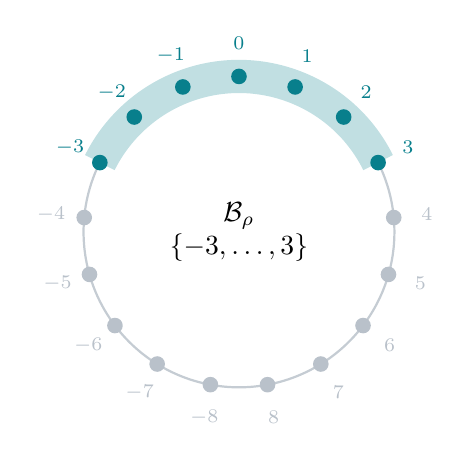
\begin{tikzpicture}[scale=.94]
\draw[ink!25,thick] (0,0) circle (2.1);
\draw[teal!25,line width=12pt] ({90-360*3/17}:2.1) arc ({90-360*3/17}:{90+360*3/17}:2.1);
\foreach \n in {-8,...,8}{
\ifnum\n>-4\ifnum\n<4\def\pointcolor{teal}\else\def\pointcolor{ink!30}\fi\else\def\pointcolor{ink!30}\fi
\fill[\pointcolor] ({90-360*\n/17}:2.1) circle(3pt);
\node[font=\scriptsize,text=\pointcolor] at ({90-360*\n/17}:2.55) {$\n$};}
\node[align=center] at (0,0) {$\bb_\rho$\\$\{-3,\ldots,3\}$};
\end{tikzpicture}
\column{.56\textwidth}
\[B([n],[m])=\alpha nm\in\R\qquad(|n|,|m|<17\rho).\]
\centering
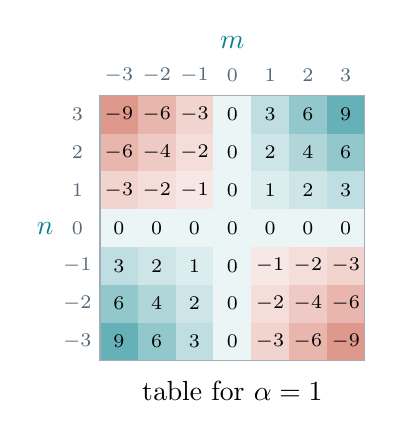
\begin{tikzpicture}[scale=.48]
\foreach \i in {-3,...,3}{\foreach \j in {-3,...,3}{
\pgfmathtruncatemacro{\val}{\i*\j}
\pgfmathtruncatemacro{\shade}{8+6*abs(\val)}
\ifnum\val<0\fill[coral!\shade] (\i,\j) rectangle +(1,1);\else\fill[teal!\shade] (\i,\j) rectangle +(1,1);\fi
\node[font=\scriptsize] at (\i+.5,\j+.5) {$\val$};}}
\draw[ink!40] (-3,-3) rectangle (4,4);
\foreach \n in {-3,...,3}{
\node[font=\scriptsize,text=muted] at (\n+.5,4.55) {$\n$};
\node[font=\scriptsize,text=muted] at (-3.6,\n+.5) {$\n$};}
\node[text=teal] at (.5,5.4) {$m$};
\node[text=teal] at (-4.45,.5) {$n$};
\node[below] at (.5,-3.3) {table for $\alpha=1$};
\end{tikzpicture}
\end{columns}
\source{\JT{Example 2.3}, using the unique small integer representatives.}
}{
Specialise the paper's example to seventeen points so that the picture is
literal. The Bohr set consists of residues with unique representatives
$-3,-2,-1,0,1,2,3$. Define the real-valued form by multiplying these
representatives; the table shows $\alpha=1$. It is symmetric and locally
bilinear.

Why is it locally additive? If $[n_1],[n_2],[n_1+n_2]$ all lie in this
small arc, their chosen representatives satisfy the same integer sum:
the possible error is a multiple of $17$ of absolute value less than
$3\rho\,17<17$. Thus it is zero. More generally this works with
$\rho<1/4$ and $G=\Z/N\Z$.

Use a representative map only on the small arc. The printed example's
description of a global homomorphic section $\Z/N\Z\to\Z$ cannot be
literal: no such section exists for $N>1$. Our notation avoids that error.
The table is real-valued as in the example; reduction modulo one will
connect it with Lemma 2.4 later.
}

\Slide{Carry-over prevents a global extension}{1:15}{
\begin{columns}[c]
\column{.40\textwidth}
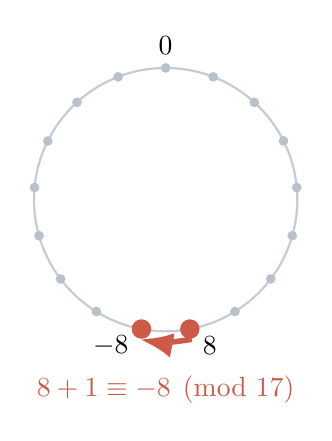
\begin{tikzpicture}[scale=.88]
\draw[ink!25,thick] (0,0) circle (1.9);
\foreach \n in {-8,...,8}{\fill[ink!30] ({90-360*\n/17}:1.9) circle(2pt);}
\fill[coral] ({90-360*8/17}:1.9) circle(4pt);
\fill[coral] ({90+360*8/17}:1.9) circle(4pt);
\draw[->,coral,line width=2pt] ({90-360*8/17}:2.05) arc ({90-360*8/17}:{90-360*9/17}:2.05);
\node[right] at ({90-360*8/17}:2.15) {$8$};
\node[left] at ({90+360*8/17}:2.15) {$-8$};
\node[below,text=coral] at (0,-2.4) {$8+1\equiv-8\pmod{17}$};
\node[above] at (0,1.95) {$0$};
\end{tikzpicture}
\column{.59\textwidth}
\small Extending the representative formula would require
\[\begin{aligned}
B([8]+[1],[1])&=-8\alpha,\\
B([8],[1])+B([1],[1])&=9\alpha.
\end{aligned}\]
\medskip
\small In fact, any global bilinear $C:G^2\to\R$ satisfies
\[17C([1],[1])=C([0],[1])=0.\]
\tagline{$\alpha\ne0$ $\Longrightarrow$ no real-valued global extension.}
\end{columns}
}{
The local formula cannot just be used with balanced representatives
everywhere. Crossing the cut from eight to minus eight changes the
integer sum by seventeen. The proposed multiplication formula therefore
fails the displayed additivity identity. These points lie outside the
local arc, so this does not contradict the local bilinearity just proved.

There is also a decisive argument against any real-valued extension,
not just this particular formula. A homomorphism from a finite group to
$\R$ is zero; bilinearity gives $17C(1,1)=C(0,1)=0$. But the local form
has $B(1,1)=\alpha$. For a $\T$-valued version the obstruction is instead
$17\alpha\notin\Z$. Do not use $\alpha=1$ modulo one as a nontrivial
counterexample: it would be the zero form. This is why the real-valued
example is useful.
}

\Slide{Unroll the circle and record the carry}{1:15}{
\[G_S=\{([n],n/17):n\in\Z\}\cong\Z.\]
\centering
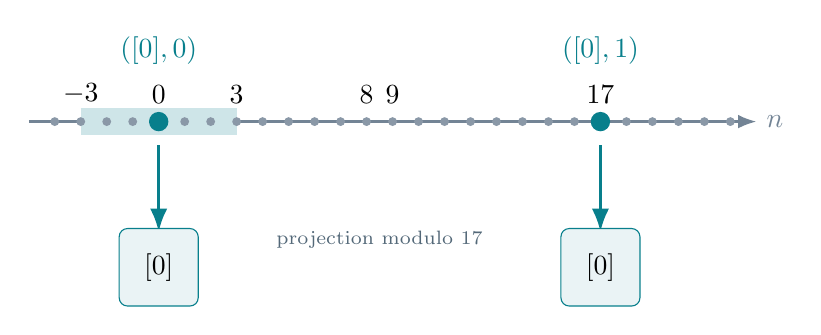
\begin{tikzpicture}[x=.33cm,y=1cm]
\draw[->,thick,ink!60] (-5,0)--(23,0) node[right] {$n$};
\draw[teal!20,line width=10pt] (-3,0)--(3,0);
\foreach \n in {-4,...,22}{\fill[ink!50] (\n,0) circle(1.6pt);}
\foreach \n in {0,17}{\fill[teal] (\n,0) circle(3.5pt);}
\foreach \n in {-3,0,3,8,9,17}{\node[above=3pt] at (\n,0) {$\n$};}
\draw[arr] (0,-.3)--(0,-1.4);\draw[arr] (17,-.3)--(17,-1.4);
\node[box] at (0,-1.85) {$[0]$};\node[box] at (17,-1.85) {$[0]$};
\node[smalllabel] at (8.5,-1.5) {projection modulo $17$};
\node[teal] at (0,.9) {$([0],0)$};\node[teal] at (17,.9) {$([0],1)$};
\end{tikzpicture}
\[([8],8/17)+([1],1/17)=([-8],9/17)\ne([-8],-8/17).\]
\[\widetilde B\bigl(([n],n/17),([m],m/17)\bigr)=\alpha nm.\]
\source{\JT{Example 2.3}. The second coordinate remembers the integer lift.}
}{
Replace a residue by the pair consisting of the residue and a real lift
of its character value. The resulting group is an infinite cyclic group,
parameterised by integers $n$. The points zero and seventeen have the
same projection, but second coordinates zero and one distinguish them.

Now eight plus one is the integer nine upstairs. It projects to minus
eight, but its height is nine-seventeenths, not minus eight-seventeenths.
The missing carry has been recorded. Multiplication $\alpha nm$ is a
globally bilinear form on this integer group. On the small highlighted
interval the canonical lift has no carry, so it agrees with the original
local form. This is the entire geometric idea of Lemma 2.2.
}

\Slide{Black box 1: globalise on the lifted group}{1:30}{
\[G_S:=\{(x,\theta)\in G\times\R^S:
\theta_\xi=\xi\cdot x\pmod1\ \ (\xi\in S)\}.\]
\begin{block}{Lemma 2.2 (Jamneshan--Tao)}
Let $G$ be a finite abelian group, $S\subseteq\Gh$, $0<r<1/2$,
and $H$ an abelian group. If
$B:\Bohr(S,r)^2\to H$ is locally bilinear, there exists a globally
bilinear map $\widetilde B:G_S^2\to H$ such that
\[\widetilde B((x,\theta),(y,\sigma))=B(x,y)
\quad\text{if }\norm{\theta}_\infty,\norm{\sigma}_\infty\leq e^{-C|S|^C}r,\]
for an absolute $C>0$. If $B$ is symmetric, $\widetilde B$ can be
chosen symmetric.
\end{block}
\tagline{A global form upstairs; agreement on a smaller neighbourhood.}
\source{\JT{Lemma 2.2}. Used as an algebraic black box.}
}{
Read the precise statement: the codomain can be any abelian group, and
symmetry is preserved. The price is an exponential shrink in the rank,
which is where the exponential radius in the final theorem originates.
The extension is on $G_S$, not on $G$.

The kernel of the projection $G_S\to G$ is $\Z^S$, and the projection
is onto, so $G_S$ is finitely generated. It need not be torsion-free:
elements of $G$ annihilated by every character in $S$ can remain as
torsion upstairs. We only need finite generation for the next lemma.
When $\norm{x}_S<r<1/2$, there is a unique lift with each real coordinate
in $(-r,r)$. On a sufficiently small neighbourhood these canonical
lifts preserve the finite sums used in local identities.
Example 2.3 explicitly constructed this extension; the general
construction is the assigned black box.
}

\Slide{Black box 2: integrate a symmetric bilinear form}{1:00}{
\begin{block}{Lemma 2.4(i) (Jamneshan--Tao)}
Let $A$ be a finitely generated abelian group. If
$\widetilde B:A\times A\to\T$ is symmetric and globally bilinear,
there exists a globally quadratic map $\widetilde\phi:A\to\T$
such that, for every $u,v\in A$,
\[\boxed{\widetilde\phi(u+v)=\widetilde\phi(u)+\widetilde\phi(v)+\widetilde B(u,v).}\]
\end{block}
\vspace{4mm}
\centering
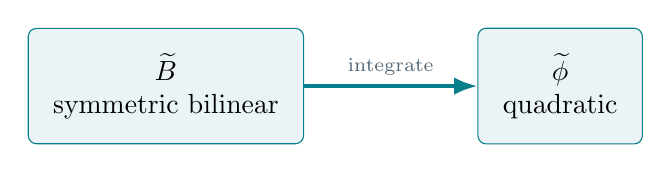
\begin{tikzpicture}
\node[box] (a) {$\widetilde B$\\symmetric bilinear};
\node[box,right=22mm of a] (b) {$\widetilde\phi$\\quadratic};
\draw[arr] (a)--node[above,smalllabel]{integrate}(b);
\end{tikzpicture}
\source{\JT{Lemma 2.4(i)}. No assumption on the parity of the torsion.}
}{
Apply this lemma to the finitely generated group $A=G_S$ from the
previous slide. It gives a quadratic primitive for every symmetric
bilinear form with values in the circle. The primitive is normalised
at zero by the identity itself. No division by two in the group is
assumed. We are black-boxing existence, as requested; the next two
slides explain the local consequence and show concrete primitives.
Do not replace this lemma by the formula $B(x,x)/2$ in $\T$: that
expression is ambiguous and can fail to respect torsion relations.
}

\Slide{Lift, integrate, restrict}{1:30}{
\begin{block}{Lemma 2.4(ii) (Jamneshan--Tao)}
Let $G$ be finite abelian, $S\subseteq\Gh$, and $r>0$.
If $B:\Bohr(S,r)^2\to\T$ is symmetric and locally bilinear,
there exist $r'$ with $\exp(-|S|^{O(1)})r\ll r'\leq r$ and
a locally quadratic map $\phi:\Bohr(S,r')\to\T$ such that
\[\phi(x+y)=\phi(x)+\phi(y)+B(x,y)
\quad(x,y\in\Bohr(S,r'/2)).\]
Moreover, $\phi$ has a globally quadratic lift
$\widetilde\phi:G_S\to\T$ agreeing with $\phi(x)$ whenever
$(x,\theta)\in G_S$ and $\norm{\theta}_\infty<r'$.
\end{block}
\[B\ \xrightarrow{\;2.2\;}\ \widetilde B
\ \xrightarrow{\;2.4(i)\;}\ \widetilde\phi
\ \xrightarrow{\;\text{small lifts}\;}\ \phi.\]
\source{\JT{Lemma 2.4(ii)}.}
}{
This is the exact local conclusion we need, including its radius loss
and the global quadratic lift. Briefly explain the three arrows rather
than proving the black boxes: globalise the form, integrate upstairs,
then restrict to unique small lifts.

Choose a smaller regular radius $r_1$ so that $\phi$ is available on
$\Bohr(S,2r_1)$ and the polarisation identity holds for
$y,z\in\Bohr(S,r_1)$. We retain
$r_1\gg\exp(-\eta^{-O(1)})$. In applications take radii safely below
$1/4$, so every parallelogram or cube in the domain lifts without carry.
This explains local quadraticity, not just the polarisation identity
for pairs based at zero.

We have not yet retained correlation on this exponentially smaller set.
Direct restriction could lose an exponential factor. The final proof
uses small translations of the original averages instead.
}

\Slide{Example 2.3: the quadratic appears upstairs}{1:30}{
\begin{columns}[c]
\column{.44\textwidth}
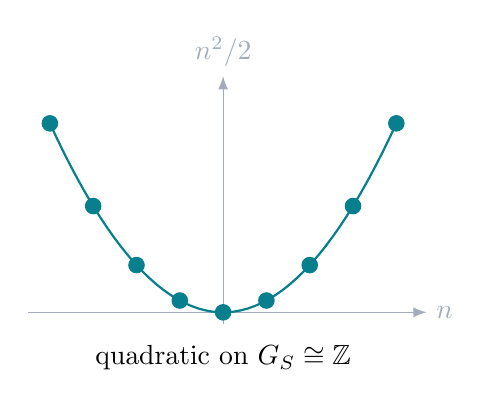
\begin{tikzpicture}[x=.55cm,y=.30cm]
\draw[->,ink!40] (-4.5,0)--(4.7,0) node[right] {$n$};
\draw[->,ink!40] (0,-.5)--(0,10) node[above] {$n^2/2$};
\draw[teal,thick,domain=-4:4,samples=50] plot (\x,{\x*\x/2});
\foreach \n in {-4,...,4}{\fill[teal] (\n,{\n*\n/2}) circle(3pt);}
\node[below] at (0,-1) {quadratic on $G_S\cong\Z$};
\end{tikzpicture}
\column{.55\textwidth}
\[\widetilde\phi(n)=\frac{\alpha n^2}{2}\pmod1\]
\[\widetilde\phi(n+m)-\widetilde\phi(n)-\widetilde\phi(m)=\alpha nm.\]
\medskip
\small A torsion check: $A=\Z/2\Z$, $B(1,1)=1/2$.
\[\phi(0)=0,\qquad\phi(1)=1/4.\]
\[0=1/4+1/4+1/2\pmod1.\]
\end{columns}
\source{Illustrations of \JT{Example 2.3 and Lemma 2.4}. The parabola shows the real lift with $\alpha=1$.}
}{
On the integer cover, the primitive is the familiar real parabola
$\alpha n^2/2$, reduced modulo one. Its second difference is exactly
$\alpha nm$. Restrict to the short integer interval to obtain the
desired local quadratic downstairs. The plotted parabola is a real lift
with $\alpha=1$; it illustrates integration, not a nontrivial
modulo-one bilinear obstruction.

The two-element example isolates the even-torsion issue. The symmetric
form with $B(1,1)=1/2$ has a quadratic primitive taking value $1/4$ at
one. Check the only nontrivial addition relation: one plus one is zero,
and the displayed sum is zero modulo one. Fourth roots of unity are
natural even though the group has exponent two. This is why the
codomain $\T$ and the correct integration lemma handle cases that a
naive field-valued quadratic formula misses. The general cyclic formula
is on a backup slide if asked.
}

\Slide{Finish the proof: move the quadratic into $f$}{2:30}{
\small Choose regular $\bb_2\ll\bb_1\ll\bb_\rho$, where
$\bb_i=\Bohr(S,r_i)$ and $r_2\asymp\poly\,r_1$.
\[(h,k)\mapsto(h+y+z,k-y),\qquad y\in\bb_1,\ z\in\bb_2.\]
\[\begin{aligned}
B(h+y+z,k-y)
={}&B(h,k)-B(h,y)+B(y+z,k)-B(y,y)\\
&-\phi(y+z)+\phi(y)+\phi(z).
\end{aligned}\]
\small Put $x'=x+h+k$, absorb terms in $y$ or $y+z$, and fix $h,k$:
\[\boxed{\abs{\E_{\substack{x'\in G\\y\in\bb_1,\ z\in\bb_2}}
a(x',y+z)b(x',y)\underbrace{f(x'+z)e(-\phi(z))}_{g_{x'}(z)}}\gg\poly.}\]
\tagline{Small shifts preserve correlation despite the small final radius.}
\source{\JT{proof of Theorem 1.6, equation (26) and subsequent changes of variables}.}
}{
Start from Lemma 2.6, still averaging $h,k$ over the original regular
Bohr set. Integrate on a much smaller domain using Lemma 2.4 and choose
regular $r_1$ with a safety margin, for instance below a sufficiently
small polynomial multiple of $\rho$. Choose $r_2$ a still smaller
polynomial multiple of $r_1$. The quadratic identity is valid for all
$y\in\bb_1,z\in\bb_2$, and all sums in the display are in the original
doubled domain.

Average the small translations $(h,k)\mapsto(h+y+z,k-y)$. Regularity
bounds the error; the argument of $f$ becomes $x+h+k+z$. Expand the
bilinear phase as displayed. The crucial identity is
$B(y,z)=\phi(y+z)-\phi(y)-\phi(z)$, with the signs exactly as shown.
After inserting the minus sign in $e(-B)$, every term except
$-\phi(z)$ depends on $y$ or on $y+z$, with $x,h,k$ held fixed.
Absorb those terms into the two separate bounded factors.

Set $x'=x+h+k$, then fix $h,k$ retaining a large average. We obtain
the box. We never divided by the global density of the tiny Bohr sets;
that is why the correlation remains polynomial.
}

\Slide{One local Fourier coefficient removes the last factors}{2:30}{
\begin{block}{Local Fourier extraction (Green--Tao, Lemma 4.4)}
Let $P,Q$ be nonempty subsets of a finite abelian group $G$,
$g:G\to\C$, and $a,b:G\to\C$ be 1-bounded. Then
\[\sup_{\xi\in\Gh}\abs{\E_{z\in Q}g(z)e(-\xi\cdot z)}
\geq\frac{|P|}{|P+Q|}
\abs{\E_{y\in P,\,z\in Q}a(y+z)b(y)g(z)}.\]
\end{block}
\small Use $P=\bb_1$, $Q=\bb_2$, $g(z)=f(x+z)e(-\phi(z))$.
Regularity gives $|\bb_1+\bb_2|\leq2|\bb_1|$.
\[\boxed{\E_x\abs{\E_{z\in\bb_2}f(x+z)e(-\phi(z)-\xi(x)\cdot z)}\gg\poly.}\]
\source{\GT{Lemma 4.4}. Fourier expansion and Cauchy--Schwarz prove the stated inequality.}
}{
State the lemma, then explain its short proof; it is not an additional
unexplained black box. Extend $g\mathbf1_Q$, $b\mathbf1_P$ and
$a\mathbf1_{P+Q}$ by zero on $G$. Fourier expansion writes the
trilinear average as a sum of a product of their three Fourier transforms,
divided by the densities of $P$ and $Q$.
Bound the transform of $g\mathbf1_Q$ by its supremum. Cauchy--Schwarz
and Parseval bound the other two transforms by
$\sqrt{|P||P+Q|}/|G|$. In fact this proves the stronger factor
$\sqrt{|P|/|P+Q|}$; the displayed weaker factor is the published lemma.

Apply pointwise in $x$ to the previous slide. Take $\xi(x)$ maximizing
the local Fourier coefficient. Averaging the resulting inequalities in
$x$ and using the triangle inequality gives the boxed conclusion.
Since $\bb_1$ is regular and $r_2/r_1$ is sufficiently small relative to
$1/|S|$, its sum with $\bb_2$ is at most twice as large.
The final average is on $\bb_2$, the domain of $z$ throughout the
argument. This also resolves the inconsistent radius label in the last
display of the printed proof.
}

\Slide{Theorem 1.6 is proved}{1:15}{
\centering
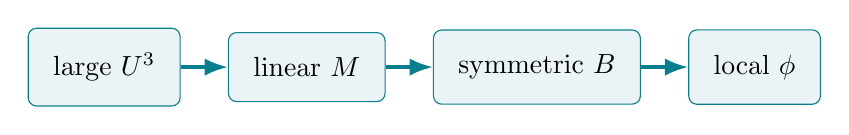
\begin{tikzpicture}[node distance=6mm]
\node[box] (a) {large $U^3$};
\node[box,right=of a] (b) {linear $M$};
\node[box,right=of b] (c) {symmetric $B$};
\node[box,right=of c] (d) {local $\phi$};
\draw[arr] (a)--(b);\draw[arr] (b)--(c);\draw[arr] (c)--(d);
\end{tikzpicture}
\vspace{3mm}
\[\E_x\abs{\E_{h\in\Bohr(S,r_2)}f(x+h)e(-\phi(h)-\xi(x)\cdot h)}\gg\poly.\]
\vspace{1mm}
\begin{tabular}{ll}
\textcolor{teal}{Rank} & $|S|\ll\eta^{-O(1)}$\\[3mm]
\textcolor{teal}{Radius} & $\exp(-\eta^{-O(1)})\ll r_2\leq1/100$\\[3mm]
\textcolor{teal}{Correlation} & $\gg\eta^{O(1)}$
\end{tabular}
\tagline{The lift records carries. Integration handles all torsion.}
}{
Check the quantitative conclusions once. The graph and symmetry steps add
only polynomially many frequencies. All radius losses before integration
are polynomial. Lemma 2.2, through Lemma 2.4, contributes the exponential
shrink $\exp(-|S|^{O(1)})$; the final polynomial shrink preserves the
required exponential lower bound. Choose the final regular radius below
$1/100$. The correlation has only polynomial losses throughout, because
we used averaged translations and pointwise Fourier extraction rather
than direct restriction to a tiny set.

The two lessons are concrete: the combinatorial work turns a noisy graph
into a locally linear frequency map, and the lifted group remembers
carry-over so a symmetric bilinear form can be integrated in arbitrary
torsion. Stop here. The remaining slides are references and optional
backup material, not part of the timed talk.
}

\Slide{References and where to look}{not timed}{
\small
\textbf{[JT] A. Jamneshan and T. Tao.}\par
\emph{The inverse theorem for the $U^3$ Gowers uniformity norm on arbitrary
finite abelian groups: Fourier-analytic and ergodic approaches.}\par
Discrete Analysis 2023:11.
\href{https://arxiv.org/abs/2112.13759}{arXiv:2112.13759v3}.\par
\textcolor{teal}{Theorem 1.6; Lemmas 2.2, 2.4--2.6; Example 2.3.}\par
\medskip
\textbf{[GT] B. Green and T. Tao.}\par
\emph{An inverse theorem for the Gowers $U^3(G)$ norm.}\par
Proc. Edinb. Math. Soc. (2) 51 (2008), 73--153.
\href{https://arxiv.org/abs/math/0503014}{arXiv:math/0503014v4}.\par
\textcolor{teal}{\S5: energy and BSG; \S9: graph and symmetry; Lemmas 4.4, 6.3, 8.4, 8.8.}\par
\medskip
\textbf{[Green] B. Green.}\par
\emph{Montr\'eal lecture notes on quadratic Fourier analysis.}
\href{https://arxiv.org/abs/math/0604089}{arXiv:math/0604089v2}.\par
\textcolor{teal}{\S2: the $\F_5^n$ model, especially Propositions 2.5--2.6 and Lemma 2.8.}
}{
Leave this slide up for questions. These are the primary sources consulted
for the proof. The preparation appendix maps each imported input to its
exact lemma or proposition and explains the finite-field model separately.
The older Green--Tao propositions are used with the explicit Jamneshan--Tao
modification removing the factor two. Green--Tao's December 2023 correction
to Proposition 3.2 does not affect the inputs used here; we never invoke
that extension claim.
}

\Backup{regular Bohr sets and translation errors}{}{
\begin{block}{Regularity and regular radii}
Write $d=\max(1,|S|)$. A Bohr set $P=\Bohr(S,r)$ is regular if
\[(1-100d|\kappa|)|P|\leq|\Bohr(S,(1+\kappa)r)|
\leq(1+100d|\kappa|)|P|\]
for $|\kappa|\leq1/(100d)$. For every $0<\varepsilon<1$ there
exists $r\in[\varepsilon,2\varepsilon]$ with $\Bohr(S,r)$ regular.
\end{block}
\small If $P$ is regular, $|F|\leq1$, and $\norm{t}_S\leq\varepsilon r$
with $\varepsilon\leq1/(100d)$, then
\[\abs{\E_{x\in P}F(x+t)-\E_{x\in P}F(x)}\leq200d\varepsilon.\]
\source{\GT{Definition 2.6, Lemmas 8.2 and 4.2}. Existence of regular radii is a standard black box.}
}{
The case $S=\varnothing$ is trivial: the Bohr set is $G$. Otherwise the
definition agrees with the paper. The regular-radius existence theorem is
the auxiliary geometric input we use without proof.

The translation estimate follows directly: both $P$ and $P+t$ contain
$\Bohr(S,(1-\varepsilon)r)$ and are contained in
$\Bohr(S,(1+\varepsilon)r)$. Thus the symmetric difference has size
at most $200d\varepsilon|P|$. Dividing by $|P|$ proves the inequality.
For a small Bohr set $Q=\Bohr(S,s)$, the inclusion
$P+Q\subseteq\Bohr(S,r+s)$ also gives $|P+Q|\leq2|P|$ when
$s/r\leq1/(100d)$. These are precisely the boundary estimates used
in the symmetry and final Fourier steps.
}

\Backup{the finite-field model for Lemma 2.5}{}{
\small Take $G=\F_5^n$ and identify $\Gh$ with $\F_5^n$.
\begin{center}
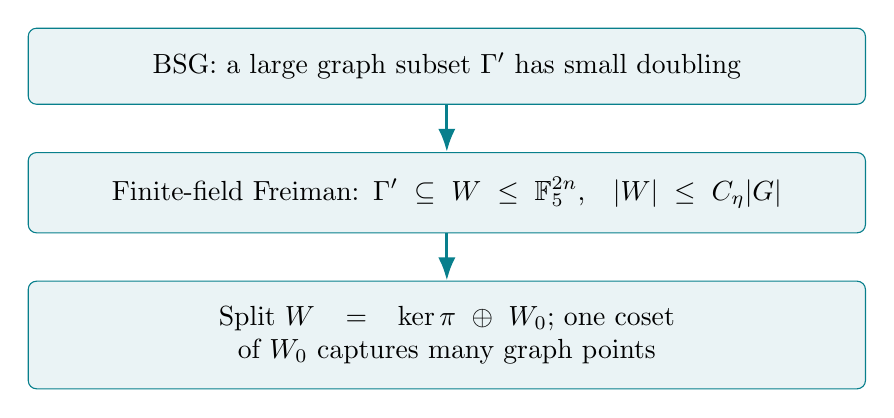
\begin{tikzpicture}[node distance=6mm]
\node[box,text width=10cm] (a) {BSG: a large graph subset $\Gamma'$ has small doubling};
\node[box,text width=10cm,below=of a] (b) {Finite-field Freiman: $\Gamma'\subseteq W\leq\F_5^{2n}$,\quad $|W|\leq C_\eta|G|$};
\node[box,text width=10cm,below=of b] (c) {Split $W=\ker\pi\oplus W_0$; one coset of $W_0$ captures many graph points};
\draw[arr] (a)--(b);\draw[arr] (b)--(c);
\end{tikzpicture}
\end{center}
\[\pi|_{W_0}\text{ injective}\quad\Longrightarrow\quad
\xi_h=Lh+\xi_0\text{ on a large subset}.\]
\source{\Green{Proposition 1.14 and Proposition 2.6}. This qualitative shortcut is a model, not the quantitative proof above.}
}{
Green's notes offer a simpler finite-field route. The input finite-field
Freiman theorem says: for fixed $p$ and $K$, a finite nonempty
$A\subseteq\F_p^m$ with $|A+A|\leq K|A|$ is contained in a subspace
of size at most $C_{p,K}|A|$. We apply it to $\Gamma'$ in $\F_5^{2n}$.
The projection of the resulting subspace $W$ contains a set of size
$c_\eta|G|$, so $|\ker(\pi|_W)|=|W|/|\pi W|\leq C_\eta$.

Choose a vector-space complement $W_0$ to this kernel. Projection is
injective on each coset of $W_0$; there are only $C_\eta$ cosets inside
$W$. One therefore contains many points of $\Gamma'$. Its inverse
projection is affine, giving $\xi_h=Lh+\xi_0$ on that subset. Extend
$L$ from its subspace to all of $G$ using a basis if needed.

This clarifies the geometry, but these qualitative constants do not
establish the polynomial correlation bound needed in the main theorem.
For those bounds use the graph-refinement/Bogolyubov route, even in
finite fields. Also, a small-radius Bohr set in $\F_p^n$ is an intersection
of kernels, so the corresponding local map is an ordinary linear map.
}

\Backup{Bogolyubov in four Fourier lines}{}{
\small Let $|A|=\delta|G|$, and use normalised convolution.
\[F:=\mathbf1_A*\mathbf1_A*\mathbf1_{-A}*\mathbf1_{-A},
\qquad\supp F\subseteq2A-2A.\]
\[F(x)=\sum_{\xi\in\Gh}|\widehat{\mathbf1_A}(\xi)|^4 e(\xi\cdot x).\]
\[S:=\{\xi:|\widehat{\mathbf1_A}(\xi)|\geq\delta^{3/2}/\sqrt2\},
\qquad |S|\leq2\delta^{-2}.\]
\[x\in\Bohr(S,1/4)\quad\Longrightarrow\quad
F(x)\geq\delta^4-\frac{\delta^3}{2}\sum_\xi|\widehat{\mathbf1_A}(\xi)|^2
=\frac{\delta^4}{2}>0.\]
\tagline{Positive convolution $\Longrightarrow$ an additive representation.}
\source{\GT{Lemma 6.3}.}
}{
This is the proof of the global Bogolyubov statement used in Lemma 2.5.
The transform of the fourfold convolution is the nonnegative fourth power
of the transform magnitude. The zero frequency contributes $\delta^4$.
For every other large frequency, a point in the Bohr set makes the real
part of its character nonnegative. The remaining frequencies have total
fourth-power mass at most $(\delta^3/2)\delta$, by Parseval. The resulting
strictly positive value implies that $x$ has a representation as a sum
of two elements of $A$ minus two others. Parseval also bounds the number
of large frequencies, giving the rank estimate. The subtle local version
in slide 15 replaces global Parseval counting with a local Bessel estimate;
the preparation appendix spells out that replacement.
}

\Backup{local Fourier decay}{}{
\begin{block}{Green--Tao, Lemma 8.4}
Let $U=\Bohr(S,r)$ be regular, $d=\max(1,|S|)$, and
$\ell:\Bohr(S,2r)\to\T$ satisfy
$\ell(x+y)=\ell(x)+\ell(y)$ for $x,y\in U$.
If $|\E_{x\in U}e(\ell(x))|\geq\tau>0$, then
\[\norm{\ell(t)}_{\T}\leq\frac{2^{12}d}{r\tau^2}\norm{t}_S
\qquad(t\in U).\]
\end{block}
\[L\asymp\frac{\tau r}{d\norm{t}_S},\qquad
\frac\tau2\leq\abs{\E_{|j|\leq L}e(j\ell(t))}
\ll\frac1{L\norm{\ell(t)}_{\T}}.\]
\source{\GT{Lemma 8.4}. Regularity gives the first inequality; a geometric series gives the second.}
}{
Take $L$ to be the largest integer with
$L\norm{t}_S\leq\tau r/(400d)$. If $L=0$, the stated bound is trivial
because the right side already exceeds the possible circle distance.
Otherwise the shifts $jt$, $|j|\leq L$, change the mean by at most
$\tau/2$. Local additivity gives
$\ell(x+jt)=\ell(x)+j\ell(t)$, with every intermediate multiple
remaining in the allowed domain. Factor the shifted average and use
that the original mean has magnitude at most one. The normalised
geometric sum in $j$ must have magnitude at least $\tau/2$.
Its usual upper bound gives the displayed conclusion. If
$\norm{t}_S=0$, arbitrary $L$ are allowed, which forces
$\ell(t)=0$ in $\T$. This handles the kernel of the Bohr seminorm.
}

\Backup{integrating on a cyclic group of any order}{}{
\small If $B:(\Z/N\Z)^2\to\T$ is globally bilinear, then
\[B([n],[m])=\frac{a nm}{N}\pmod1\qquad(a\in\Z).\]
\[\boxed{\phi([n])=\frac{a\,n(n-N)}{2N}\pmod1.}\]
\[\phi(n+N)-\phi(n)=an\in\Z\]
\[\phi(n+m)-\phi(n)-\phi(m)=\frac{a nm}{N}\pmod1.\]
\tagline{The linear correction enforces periodicity, even when $N$ is even.}
\source{\JT{proof of Lemma 2.4(i)}, rewritten from its binomial-coefficient formula.}
}{
This optional calculation explains the algebra behind the integration
black box on cyclic groups. Bilinearity forces $B(1,1)$ to be
$N$-torsion in $\T$, so it equals $a/N$. The displayed primitive is
$an^2/(2N)-an/2$. The linear term does not affect the polarisation,
but makes the primitive $N$-periodic: replacing $n$ by $n+N$ adds
the integer $an$. This works for both odd and even $N$.

For $\Z$, use $\alpha n^2/2$. For a product of groups, sum the
primitives on individual factors and add one cross term for each pair
of distinct factors. Symmetry makes this polarise to the full bilinear
form. The structure theorem for finitely generated abelian groups then
proves Lemma 2.4(i). This derivation is for preparation or questions;
the assignment allows the lemma itself to be black-boxed in the talk.
}

\clearpage
\section*{Preparation appendix: the arguments behind the notes}
This appendix is for rehearsal and questions. The timed talk is complete
at slide 27. The proof below uses the source notation only where useful;
in particular $M$ is never defined by dividing a character by two.

\subsection*{1. Source map and scope of the black boxes}
\begin{center}\small
\begin{tabular}{>{\raggedright\arraybackslash}p{.29\linewidth}>{\raggedright\arraybackslash}p{.35\linewidth}>{\raggedright\arraybackslash}p{.27\linewidth}}
Input & Exact source & Treatment\\\hline
Derivative frequencies and graph energy & \GT{Proposition 5.1} & Proved, slides 7--8\\
BSG and Pl\"unnecke & \GT{Theorems 5.2--5.3} & Stated black boxes, slide 9\\
Separation and graph refinement & \GT{Lemmas 8.3, 9.2} & Explained, slide 10\\
Global Bogolyubov & \GT{Lemma 6.3} & Stated, slide 11; proof in backup\\
Recovering correlation & \GT{Propositions 9.1, 9.3}; \JT{Lemma 2.5} & Proved, slides 11--12\\
Regular-radius existence & \GT{Lemma 8.2} & Stated black box, backup 1\\
Regularity shift estimates & \GT{Lemma 4.2} & Boundary proof in backup 1\\
Local Fourier decay & \GT{Lemma 8.4} & Proof, slide 15 notes / backup 4\\
Local Bogolyubov & \GT{Lemma 8.8} & Stated combinatorial input, slide 15; derivation below\\
Symmetry & \GT{Lemma 9.4}; \JT{Lemma 2.6} & Proved, slides 14--17\\
Lift and integrate & \JT{Lemmas 2.2, 2.4} & Stated algebraic black boxes, slides 21--23\\
Final Fourier coefficient & \GT{Lemma 4.4} & Proved, slide 26\\
Finite-field comparison & \Green{Propositions 2.5--2.6, Lemma 2.8} & Optional model, backup 2
\end{tabular}\end{center}
Here [JT] is arXiv:2112.13759v3 (2023); [GT] is arXiv:math/0503014v4
(December 2023); [Green] is arXiv:math/0604089v2 (2007). The bibliography
slide gives publication information and clickable links. The numbering in
this presentation is the main paper's numbering: the frequency-map result
is \emph{Lemma} 2.5, not Theorem 2.5. Green's notes have a different
Proposition 2.5.

\subsection*{2. The Cauchy--Schwarz calculation in slide 8}
Extend $\xi_h$ arbitrarily outside $H$ and put $F_k(h)=\mathbf1_H(h)e(\xi_h\cdot k)$.
For $a_h(x)=f(x+h)\overline{f(x)}$, squaring the Fourier coefficient gives
\[
|\widehat a_h(\xi_h)|^2
=\E_{x,k}f(x+h)\overline{f(x+h+k)}\overline{f(x)}f(x+k)e(\xi_h\cdot k).
\]
Thus, with $u(x,k)=f(x)\overline{f(x+k)}$ and
$v(x,k)=\overline{f(x)}f(x+k)$,
\[
\delta_0:=\E_h\mathbf1_H(h)|\widehat a_h(\xi_h)|^2
=\E_{x,h,k}u(x+h,k)v(x,k)F_k(h)\geq\eta^{16}/4.
\]
Since $|v|\leq1$, Cauchy--Schwarz gives
\[
\delta_0^2\leq
\E_{x,k}\abs{\E_hu(x+h,k)F_k(h)}^2
=\E_{y,a,k}u(y,k)\overline{u(y+a,k)}
       \E_hF_k(h)\overline{F_k(h+a)}.
\]
Here $y=x+h$ and $a$ is the difference of the two copies of $h$.
The right side is real and nonnegative before rearrangement. Since the
bounded factor is independent of $h$, a second Cauchy--Schwarz yields
\[
\delta_0^4\leq
\E_{a,k}\abs{\E_hF_k(h)\overline{F_k(h+a)}}^2
=\E_{h,a,b,k}F_k(h)\overline{F_k(h+a)}
                  \overline{F_k(h+b)}F_k(h+a+b).
\]
Average over $k$ using character orthogonality. The result is exactly the
normalised count of parallelograms in $H$ whose four frequencies obey the
same alternating relation. It is at least $\eta^{64}/256$. There are
$|G|^3$ ordered base parallelograms, proving the energy estimate with the
correct normalisation. This argument works for complex 1-bounded $f$ and
does not need the real-valued Samorodnitsky identity used in Green's notes.

\subsection*{3. Why the graph refinement has polynomial cost}
After BSG and Pl\"unnecke, enlarge $K\ll\eta^{-O(1)}$ until
$|\Gamma'|\geq |G|/K$ and $|9\Gamma'-8\Gamma'|\leq K|G|$.
Define
\[V=\{v\in\Gh:(0,v)\in8\Gamma'-8\Gamma'\}.\]
For each first coordinate of $\Gamma'$, adding all of $V$ produces
$|V|$ different points. Therefore
\[|\Gamma'||V|=|\Gamma'+(\{0\}\times V)|\leq K|G|,
\qquad |V|\leq K^2.\]
Characters on $\Gh$ are evaluations at elements of $G$, by finite
Pontryagin duality. If $v\ne0$, a uniformly random character $s$ of
$\Gh$ has $s(v)$ uniform on a nontrivial finite cyclic subgroup of
$\T$. At most two thirds of that subgroup lies in $(-1/4,1/4)$.
Successively choose a character leaving at most two thirds of the surviving
nonzero elements of $V$. After $O(\log(2|V|))$ choices,
\[V\cap\{v:\norm{s(v)}_\T<1/4\text{ for every chosen }s\}=\{0\}.\]
Let $m$ be the number of tests and $\Psi:\Gh\to\T^m$ their product.
Partition the torus into $128^m$ cubes of side $1/128$, using
representatives in $[0,1)^m$. Choose a cube containing at least this
fraction of the frequencies of $\Gamma'$ and call the resulting graph
$\Gamma''$. Since $m=O(\log K)$, its size is at least
$K^{-O(1)}|G|$.

If $(0,v)\in8\Gamma''-8\Gamma''$, then $v\in V$. In each tested
coordinate the eight positive and eight negative cube origins cancel;
the remaining real sum has magnitude below $16/128<1/4$.
Thus $v=0$. If two points of $4\Gamma''-4\Gamma''$ share a first
coordinate, their difference is such a vertical vector, so the two
points coincide. This proves injectivity of projection on that sumset.
We do \emph{not} claim that $8\Gamma''-8\Gamma''$ itself is a graph;
only its zero fibre is trivial.

\subsection*{4. From uniqueness of lifts to the full local-linearity condition}
Let $H''=\pi_G\Gamma''$ and choose $S$ by global Bogolyubov so that
$U_0=\Bohr(S,1/4)\subseteq2H''-2H''$. Define $M$ by the unique
lift $(h,M(h))\in2\Gamma''-2\Gamma''$ for $h\in U_0$.
For $h_1,h_2,h_3,h_4\in U_0$ with $h_1+h_2=h_3+h_4$, compare the
two sums of lifts in $4\Gamma''-4\Gamma''$. They have the same first
coordinate and hence the same second coordinate:
\[M(h_1)+M(h_2)=M(h_3)+M(h_4).\]
This is precisely the vanishing of all second differences. The
three-point additivity identity alone on an arbitrary subset would not
automatically imply this stronger four-point statement, so it is useful
to prove the latter directly. Also $M(0)=0$. The regular radius
$\rho\in[1/16,1/8]$ ensures $\Bohr(S,2\rho)\subseteq U_0$.

To get back to $f$, choose $x_0$ so the set
$A=\{h\in\Bohr(S,\rho):x_0+h\in H''\}$ has relative density
at least $|H''|/|G|$. Then $\xi_{x_0+h}=\xi_0+M(h)$ on $A$.
Write
\[c_h=\E_xf(x+x_0+h)\overline{f(x)}e(-[\xi_0+M(h)]\cdot x),\]
and choose $\lambda_h$ with $|\lambda_h|=1$ and
$\lambda_hc_h=|c_h|$ (choose $1$ if $c_h=0$). After $u=x+x_0$,
the explicit bounded factors can be taken as
\[
b_1(h)=\mathbf1_A(h)\lambda_h e((\xi_0+M(h))\cdot x_0),
\qquad b_2(u)=\overline{f(u-x_0)}e(-\xi_0\cdot u).
\]
This verifies both the size and the exact variable dependencies in
Lemma 2.5. No replacement of $f$ by an uncontrolled function is needed.

\subsection*{5. Symmetry: the algebra inside the Cauchy--Schwarz step}
After averaging translates, the Lemma 2.5 correlation gives
\[
\abs{\E_{h\in P,x\in U}a(h)c(x+h)b(x)e(-M(h)\cdot x)}\geq\delta,
\]
where $P$ is the original regular Bohr set, $U$ is much smaller and
regular, and $\delta\gg\eta^{O(1)}$. All points used below lie in the
original doubled domain of $M$. Squaring in $h$ introduces $x,y\in U$
and the phase $M(h)\cdot(y-x)$. Put $w=x+y+h$ and expand:
\[
\begin{aligned}
M(w-x-y)\cdot(y-x)
={}&M(w)\cdot y-M(w)\cdot x\\
&+M(x)\cdot x-M(y)\cdot y-D(x,y).
\end{aligned}
\]
Everything except $-D(x,y)$ is a sum of a function of $(w,x)$ and
a function of $(w,y)$. The factors $c(x+h)$ and
$\overline{c(y+h)}$ become $c(w-y)$ and $\overline{c(w-x)}$,
which have the same separated dependencies. Replace $P+x+y$ by $P$
using regularity, losing $O(d\,\operatorname{rad}(U)/\operatorname{rad}(P))$.
Fix $w$ by averaging and, if necessary, interchange $x,y$. Then
\[\abs{\E_{x,y\in U}u(x)v(y)e(D(x,y))}\geq\delta_1,
\qquad\delta_1\gg\eta^{O(1)}.\]
One more Cauchy--Schwarz gives
\[\E_{y,y'\in U}\abs{\E_{x\in U}e(D(x,y-y'))}\geq\delta_1^2.\]
There is a $y_0$ and a subset $A\subseteq U$ of relative density
$\gg\delta_1^2$ for which each inner absolute value with $y'=y_0$
is $\gg\delta_1^2$. Apply local Fourier decay to obtain
\[\norm{D(t,y_0-y)}_\T\ll\eta^{-O(1)}\norm{t}_S
\quad(t\in U,\ y\in A).\]
For $z=a_1+a_2-a_3-a_4\in2A-2A$, write
\[z=(y_0-a_3)+(y_0-a_4)-(y_0-a_1)-(y_0-a_2).\]
Bilinearity and the triangle inequality yield the same estimate with a
factor four. The ambient Bohr set was chosen sufficiently small that all
partial sums needed here lie in the original domain.

Local Bogolyubov now produces $S_*=S\cup T$ of polynomial size and a
radius $r_*\gg\eta^{O(1)}$ such that
$\Bohr(S_*,r_*)\subseteq U\cap(2A-2A)$. Consequently
\[\norm{D(t,z)}_\T\leq L\norm{t}_{S_*},\qquad L\ll\eta^{-O(1)},\]
for both variables in that Bohr set. Shrink to $2r\leq\varepsilon/L$
and $2r\leq r_*$, with $r$ regular and $\varepsilon$ a sufficiently
small power of $\eta$. This makes the real-midpoint argument valid on
the whole doubled Bohr set needed in Lemma 2.6.

\subsection*{6. Why local Bogolyubov has polynomial parameters}
This is the extra additive-combinatorial ingredient in the symmetry
step. Here is the mechanism of \GT{Lemma 8.8}, with constants suppressed
but the density dependence retained.

Let $U=\Bohr(S,r)$ be regular, $d=\max(1,|S|)$,
$A\subseteq U$, and $|A|=\delta|U|$. Take a regular
$U'=\Bohr(S,r')$ with $r'\asymp\delta r/d$, sufficiently small that
the regularity error is at most $\delta/2$. Averaging over translates
$x+U'$, $x\in U$, gives some $x_0$ for which
\[A'=A\cap(x_0+U'),\qquad |A'|\geq(\delta/2)|U'|.\]
Use $\beta=|U|/|G|$, $\beta'=|U'|/|G|$ and normalised convolution.
The function $\mathbf1_A*\mathbf1_{A'}$ is supported in
$x_0+U+U'$, of size at most $2|U|$. Cauchy--Schwarz and Parseval give
\[
F(0):=\sum_\xi|\widehat{\mathbf1_A}(\xi)|^2
                         |\widehat{\mathbf1_{A'}}(\xi)|^2
\geq\frac{\delta^4\beta(\beta')^2}{8}.
\]
The function
$F=\mathbf1_A*\mathbf1_{A'}*\mathbf1_{-A}*\mathbf1_{-A'}$
is supported in $2A-2A$. Define
\[R=\{\xi:|\widehat{\mathbf1_{A'}}(\xi)|\geq
                       (\delta^{3/2}/8)\beta'\}.\]
The Fourier mass outside $R$ is at most
$\delta^4\beta(\beta')^2/64$. Therefore, whenever
$\norm{\xi\cdot x}_\T<1/10$ for every $\xi\in R$,
\[
F(x)\geq\tfrac12F(0)-2\sum_{\xi\notin R}
|\widehat{\mathbf1_A}(\xi)|^2|\widehat{\mathbf1_{A'}}(\xi)|^2>0.
\]
It remains to enforce these possibly numerous frequency constraints with
only polynomially many new characters. That is the role of the local
Bessel inequality.

\textbf{Local Bessel input, exact claim.}
If $V=\Bohr(S,s)$ is regular, $E\subseteq V$, and
\[\mathcal R=\{\xi:|\widehat{\mathbf1_E}(\xi)|\geq t|V|/|G|\},\]
then, for $0<\theta,t\leq1$, there exist at most $2/t^2$ frequencies
$\xi_1,\ldots,\xi_m$ such that each $\xi\in\mathcal R$ satisfies
\[\sup_{x\in\Bohr(S,\theta s)}
\norm{(\xi-\xi_j)\cdot x}_\T\leq2^{16}\theta d/t^4
\quad\text{for some }j.\]
This is \GT{Corollary 8.7}. To see its proof, choose a maximal set of
frequencies separated by $q=2^{16}\theta d/t^4$ in this seminorm.
Local Fourier decay (applied to differences of characters) bounds the
off-diagonal inner products on $V$ by
$2^6(\theta d/q)^{1/2}\leq t^2/4$.
Choose phases aligning the correlations with $\mathbf1_E$.
Cauchy--Schwarz gives
\[t^2m^2\leq\E_{x\in V}\abs{\sum_{j=1}^m c_j e(\xi_j\cdot x)}^2
\leq m+\tfrac12t^2m^2.\]
Hence $m\leq2/t^2$. Maximality ensures that these frequencies cover
the large spectrum in the displayed seminorm. This derives the input
from the local Fourier-decay lemma, rather than invoking an additional
structural theorem.

Apply it to $E=A'-x_0\subseteq U'$; translation preserves Fourier
magnitudes. With $t=\delta^{3/2}/8$, there are
$m=O(\delta^{-3})$ representative frequencies. Set
$\theta=c\delta^6/d$ sufficiently small that the approximation error
is below $1/20$. On a Bohr set enforcing $\norm{\xi_j\cdot x}<1/20$
and the old constraints at radius $\theta r'$, every frequency in $R$
has circle norm below $1/10$. Thus the positive-convolution argument
puts this Bohr set inside $2A-2A$.

Since $r'\asymp\delta r/d$, this elementary tracking yields the slightly
weaker but fully sufficient radius $c\delta^7r/d^2$, with
$O(\delta^{-3})$ new characters. \GT{Lemma 8.8} states the sharper
$c\delta^6r/d$ radius quoted on slide 15. The talk may use that stated
black box; the derivation here proves a polynomial-radius version from
scratch, which is all the symmetry argument needs. In particular, no
global density such as $|A|/|G|$ enters the rank bound.

\subsection*{7. The midpoint is exactly bilinear, not approximately so}
On the small doubled domain, choose $d(y,z)\in(-\varepsilon,\varepsilon)$
lifting $D(y,z)$, with $\varepsilon<1/10$. Whenever $y_1,y_2,y_1+y_2,z$
are in the domain,
\[d(y_1+y_2,z)-d(y_1,z)-d(y_2,z)\in\Z\cap(-3\varepsilon,3\varepsilon)=\{0\}.\]
The same holds in $z$, and $d(z,y)=-d(y,z)$. Therefore
\[B(y,z)=M(y)\cdot z-\tfrac12d(y,z)\pmod1\]
is symmetric and locally bilinear. Furthermore
\[|e(-M(y)\cdot z)-e(-B(y,z))|
=|e(-d(y,z)/2)-1|\leq\pi\varepsilon.\]
Choose $\varepsilon$ below a small fixed fraction of the current
correlation lower bound. The phase replacement then loses at most half
that bound. The fact that $d$ is a small \emph{real} lift is indispensable:
there is no globally consistent half-map on $\T$.

\subsection*{8. Lifting and integration: check the local domains}
For $r<1/2$, each $x\in\Bohr(S,r)$ has a unique lift
$\widetilde x=(x,\theta_x)$ with $\norm{\theta_x}_\infty<r$.
If $x,y,x+y$ lie in this set and $3r<1$, the integer vector
$\theta_x+\theta_y-\theta_{x+y}$ has norm below one, hence vanishes.
Similarly, if all four vertices of a parallelogram lie in the set and
$4r<1$, their lifts satisfy the same parallelogram relation. On any cube
lying there, the lifted vertices consequently form an affine cube.
Restricting a global quadratic on $G_S$ therefore gives a locally
quadratic map in the full cube sense.

The sequence $0\to\Z^S\to G_S\to G\to0$ proves finite generation:
lift a finite generating set of $G$ and append the coordinate generators
of $\Z^S$. There may still be a finite torsion subgroup upstairs.
Lemma 2.4(i) applies without any torsion-free assumption.

For the cyclic example the cover is precisely $\Z$, and
$\widetilde B(n,m)=\alpha nm$ is real-valued. Reducing modulo one and
integrating gives $\widetilde\phi(n)=\alpha n^2/2\pmod1$.
For a genuinely nontrivial circle-valued local obstruction on $\Z/17\Z$,
one may take $\alpha=\sqrt2$, so that $17\alpha\notin\Z$.

\subsection*{9. The final phase bookkeeping and Fourier normalisation}
The expansion in slide 25 is worth checking once. Symmetry gives
\[
B(h+y+z,k-y)=B(h,k)-B(h,y)+B(y+z,k)-B(y,y)-B(y,z).
\]
Use $B(y,z)=\phi(y+z)-\phi(y)-\phi(z)$. With the minus sign in the
exponential, one can assign the factors explicitly:
\[
\begin{aligned}
a_{x,h,k}(y+z)&=b_1(x,h+y+z)e(-B(y+z,k)+\phi(y+z)),\\
b_{x,h,k}(y)&=b_2(x,k-y)e(B(h,y)+B(y,y)-\phi(y)-B(h,k)).
\end{aligned}
\]
The remaining factor is exactly $f(x+h+k+z)e(-\phi(z))$.
Thus no unwanted function depending only on $z$ is hidden in $b$.
After $x'=x+h+k$ and pigeonholing $h,k$, the desired factorisation holds.

For the final Fourier lemma let $p=|P|/|G|$, $q=|Q|/|G|$ and
$r=|P+Q|/|G|$. Extend
$F=g\mathbf1_Q$, $B=b\mathbf1_P$, $A=a\mathbf1_{P+Q}$ by zero.
Then, with the normalised transform convention,
\[
I:=\E_{y\in P,z\in Q}b(y)a(y+z)g(z)
=\frac1{pq}\sum_\xi\widehat F(\xi)\widehat B(\xi)\widehat A(-\xi).
\]
Cauchy--Schwarz and Parseval yield
\[
|I|\leq\frac{\sup_\xi|\widehat F(\xi)|}{pq}\sqrt{pr}
=\sqrt{r/p}\sup_\xi\abs{\E_{z\in Q}g(z)e(-\xi\cdot z)}.
\]
Since $r\geq p$, this implies the weaker factor $p/r$ stated in
\GT{Lemma 4.4}. Apply to $P=\bb_1$, $Q=\bb_2$ for each $x$.
If the previous joint average has magnitude $\geq\delta$, then
\[\E_x\sup_\xi\abs{\E_{z\in\bb_2}g_x(z)e(-\xi\cdot z)}
\geq\tfrac12\E_x|I_x|\geq\delta/2.\]
Choose a maximizer $\xi(x)$ (the dual group is finite). This avoids
an unnecessary extra pigeonhole step and proves the exact conclusion.

\subsection*{10. Reading cautions and quantitative bookkeeping}
The following are mathematical clarifications for preparation, not
digressions to deliver in the talk.
\begin{itemize}
\item In the printed \JT{Example 2.3}, an integer representative map
is described as a homomorphic section. For $N>1$, a homomorphism
$\Z/N\Z\to\Z$ is zero, so no such section exists. Use the unique
small representative locally, or an arbitrary set-theoretic section
globally. The example and the lifting argument then work exactly as
illustrated.
\item \GT{Propositions 9.1 and 9.3} write the graph as $(h,2M(h))$;
the implicit odd-order assumption is explicitly identified and removed
in \JT{Lemma 2.5, footnote 6}. We construct $(h,M(h))$ directly.
The final doubling manoeuvre in \GT{Lemma 9.4} is likewise omitted.
\item In \GT{Proposition 9.1}, the lift belongs to
$2\Gamma''-2\Gamma''$, not $2H''-2H''$; JT footnote 7 flags this
typo. The comparison of two pair sums requires the already proved
graph property of $4\Gamma''-4\Gamma''$, not a claim that
$8\Gamma''-8\Gamma''$ is a graph.
\item The last Fourier display in the printed JT proof uses the
$\rho_1$ label, although the extracted variable $z$ is averaged over
$\Bohr(S,\rho_2)$ in the preceding trilinear form. The application of
\GT{Lemma 4.4} gives the coefficient on the latter set, which satisfies
all the bounds required by the theorem. The slides use $\bb_2$
consistently.
\item The December 2023 correction on the
\href{https://arxiv.org/abs/math/0503014}{Green--Tao arXiv record}
concerns Proposition 3.2, a global extension claim. It is not used here.
The needed algebraic extension is the explicitly stated JT Lemma 2.2
on the lifted group.
\end{itemize}
Every rank enlargement and correlation loss in Lemmas 2.5--2.6 is
polynomial in $1/\eta$. Before integration, all radii have polynomial
lower bounds. The exponential shrink in Lemma 2.4(ii) is compatible
with the target radius because $|S|\ll\eta^{-O(1)}$.
Choose the later radii with fixed safety margins so all shifted
variables remain in doubled domains and all regularity errors are
smaller than the retained correlation. Products and compositions of
finitely many polynomial bounds are still polynomial; multiplying
the exponential lower radius by a polynomial does not change its
allowed form. This is the extent of constant bookkeeping appropriate
for a 45-minute talk.

\end{document}
